\chapterimage{chap39.jpg}
\chapter{Summary}


\section{双曲函数}

\begin{figure}[htbp]
	\centering
	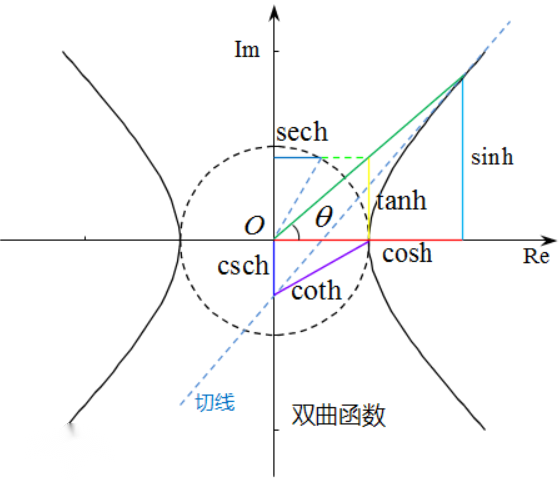
\includegraphics[width=9.5cm,height=8cm]{"figure/Summary/双曲函数.png"}
	\caption{双曲函数示意图}
	\label{Figure: 双曲函数示意图}
\end{figure} 
\begin{definition}\label{def: 双曲函数}
	双曲函数是一种类似于三角函数的一类函数,基本的函数有双曲正弦函数和双曲余弦函数,借由指数函数定义.
	
	1. 双曲正弦函数 
	$$\sinh x=\frac{e^{x}-e^{-x}}{2},x\in \mathbb{R}\quad \mathbb{R}\rightarrow \mathbb{R}$$
	
	2. 双曲余弦函数
	$$\cosh x=\frac{e^{x}+e^{-x}}{2},x\in \mathbb{R}\quad \mathbb{R}\rightarrow [1,+\infty]$$
	
	3. 双曲正切函数
	$$\tanh x=\frac{e^{x}-e^{-x}}{e^{x}+e^{-x}},x\in \mathbb{R}\quad \mathbb{R}\rightarrow (-1,1)$$
	
	恒等式:  
	$$\cosh^2 x-\sinh^2=1$$
	$$\sinh x=-i\sin ix,\quad \cosh x=\cos ix$$
	$$\sinh x=\sum\limits_{n=0}^{+\infty}\frac{x^{2n+1}}{(2n+1)!}=x+\frac{x^3}{3!}+\frac{x^5}{5!}+\dots$$
	$$\cosh x=\sum\limits_{n=0}^{+\infty}\frac{x^{2n}}{2n!}=1+\frac{x^2}{2!}+\frac{x^4}{4!}+\dots$$
\end{definition}
\begin{definition}
	反双曲函数:  
	
	1. 反双曲正弦函数
	$$\arsinh x=ln(x+\sqrt{x^2+1}),\quad (arsinh x)'=\frac{1}{\sqrt{x^2+1}}$$
	
	2. 反双曲余弦函数
	$$\arcosh x=ln(x+\sqrt{x^2-1}),\quad (arcosh x)'=\frac{1}{\sqrt{x^2-1}}$$
	
	3. 反双曲正切函数
	$$\artanh x=\frac{1}{2}ln(\frac{1+x}{1-x}),\quad (artanh x)'=\frac{1}{1-x^2}$$
\end{definition}


\section{特殊曲线}
8. 心形线、摆线、三叶玫瑰线、星形线、伯努利曲线和阿基米德螺线
\begin{definition}\label{def: 常用曲线}
	几类特殊曲线的面积、弧长、旋转体体积
	
	1.心形线 \quad $r=a(1+\cos \theta)$
	$$L=\int_{0}^{2\pi}\sqrt{a^2(1+\cos \theta)^2+a^2\sin^2\theta}d\theta=8a$$
	$$S=2\int_{0}^{\pi}a^2(1+\cos \theta)^2d\theta=\frac{3}{2}a^2\pi$$
	
	2.摆线\quad 
	$\left\lbrace
	\begin{array}{l}
		x=a(\theta-\sin \theta)\\
		y=a(1-\cos \theta)
	\end{array}
	 \right. $
	 $$L=\int_{0}^{2\pi}\sqrt{a^2(1-\cos \theta)^2+a^2\sin^2\theta}d\theta=8a$$
	 $$S=\int_{0}^{x_{0}}f(x)dx=\int_{0}^{2\pi}a^2(1-\cos \theta)^2d\theta=3a^2\pi$$
	
	3.星形线\quad $x^{\frac{2}{3}}+y^{\frac{2}{3}}=a^{\frac{2}{3}}\Leftrightarrow$
	$\left\lbrace
	\begin{array}{l}
		x=a\cos^3\theta\\
		y=a\sin^3\theta
	\end{array}
	 \right. $
	$$L=4\int_{0}^{\frac{\pi}{2}}3a\sin\theta\cos\theta d\theta=6a$$
	$$S=4\int_{0}^{\frac{\pi}{2}}3a\sin^4\theta\cos^2\theta=\frac{3\pi}{8}a^2$$
	
	4.三叶玫瑰线 \quad $\rho=a\cos 3\theta$\quad $\rho=a\sin 3\theta$
	$$L=3\int_{\frac{\pi}{6}}^{\frac{\pi}{2}}\sqrt{a^2\cos^2 3\theta+9a^2\sin^2 3\theta}d\theta=2a\int_{0}^{\frac{\pi}{2}}\sqrt{1+8\sin^2 t}dt$$
	$$S=\frac{3}{2}\int_{\frac{\pi}{6}}^{\frac{\pi}{2}}a^2\cos^2 3\theta d\theta=\frac{\pi a^2}{4}$$
	
	5.伯努利双扭线\quad $\rho^2=a^2\cos 2\theta$
	$$L=4\int_{0}^{\frac{\pi}{4}}a\sqrt{\frac{\sin^2 2\theta}{\cos 2\theta}+\cos^2 2\theta}=2a\int_{0}^{\frac{\pi}{2}}\cos^{-\frac{1}{2}}\theta d\theta$$
	$$S=2\int_{0}^{\frac{\pi}{4}}a^2\cos 2\theta d\theta=a^2$$
\end{definition}
\begin{figure}[H]
	\centering  %图片全局居中
	\subfigure[心形线]{
	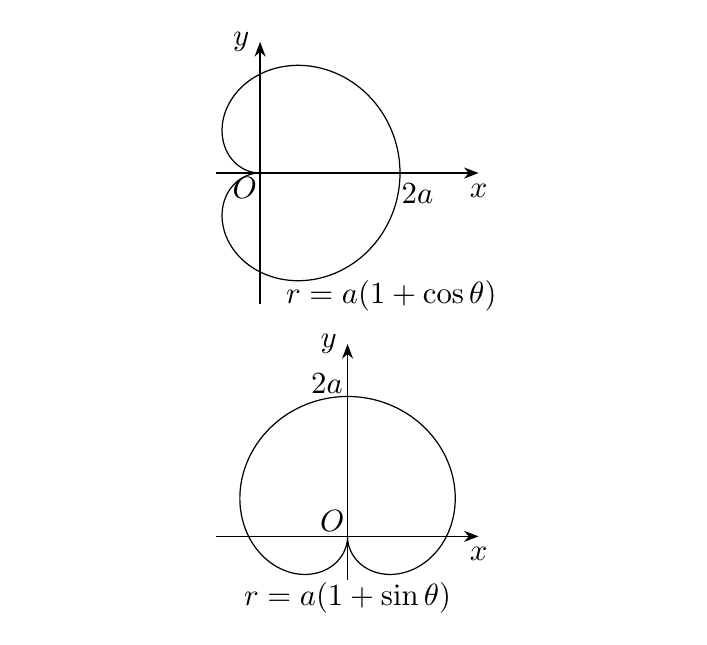
\includegraphics[width=0.45\textwidth]{"figure/Summary/心形线.png"}}
	\subfigure[摆线]{
	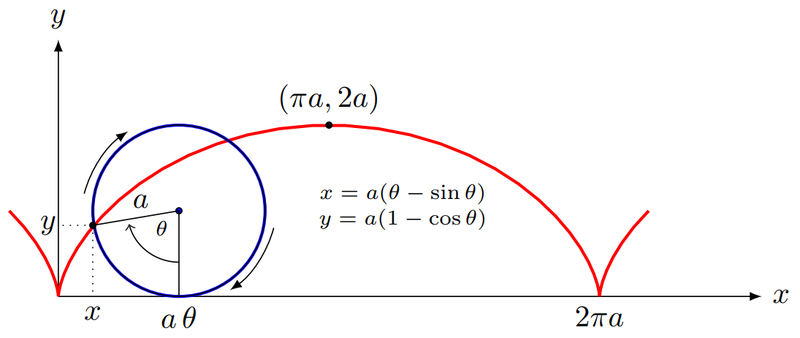
\includegraphics[width=0.45\textwidth]{"figure/Summary/摆线.png"}}
	\subfigure[星形线]{
	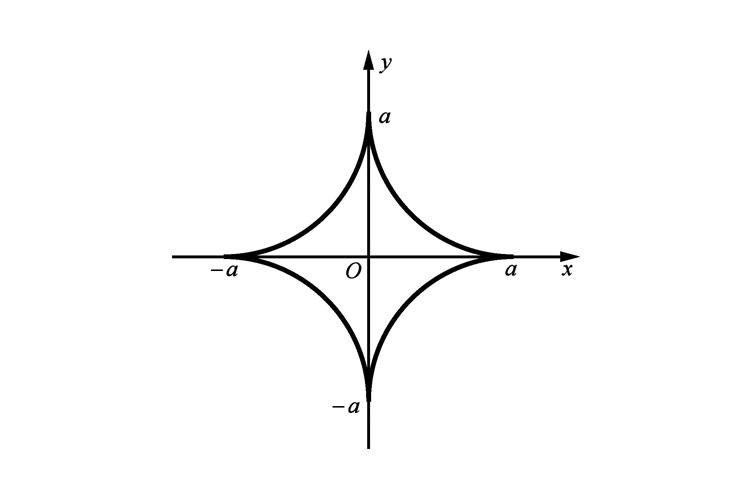
\includegraphics[width=0.45\textwidth]{"figure/Summary/星形线.jpg"}}
	\subfigure[三叶玫瑰线$\rho=a\cos 3\theta$]{
	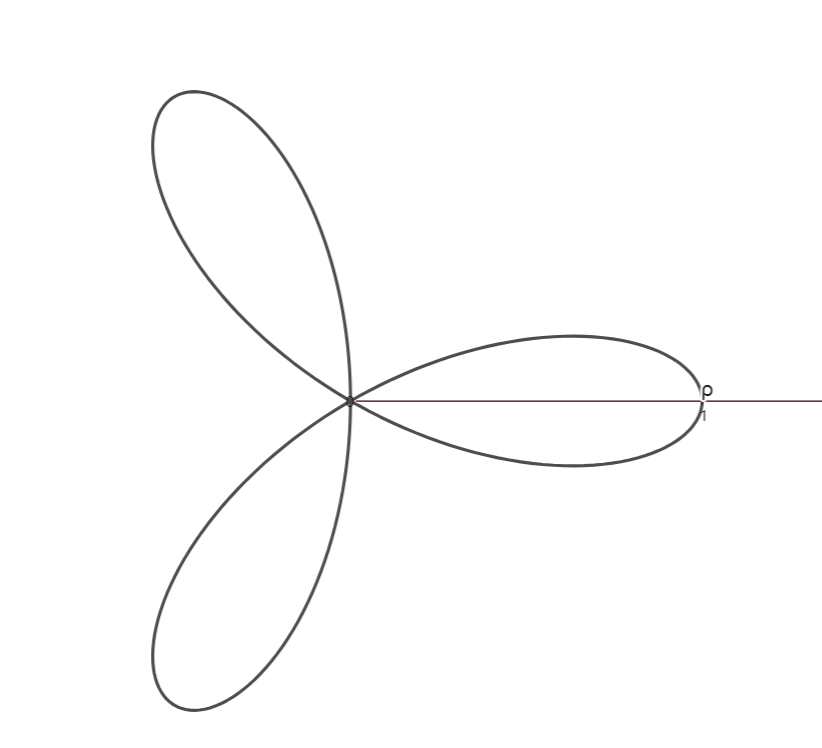
\includegraphics[width=0.45\textwidth]{"figure/Summary/三叶玫瑰线1.png"}}
	\subfigure[三叶玫瑰线$\rho=a\sin 3\theta$]{
	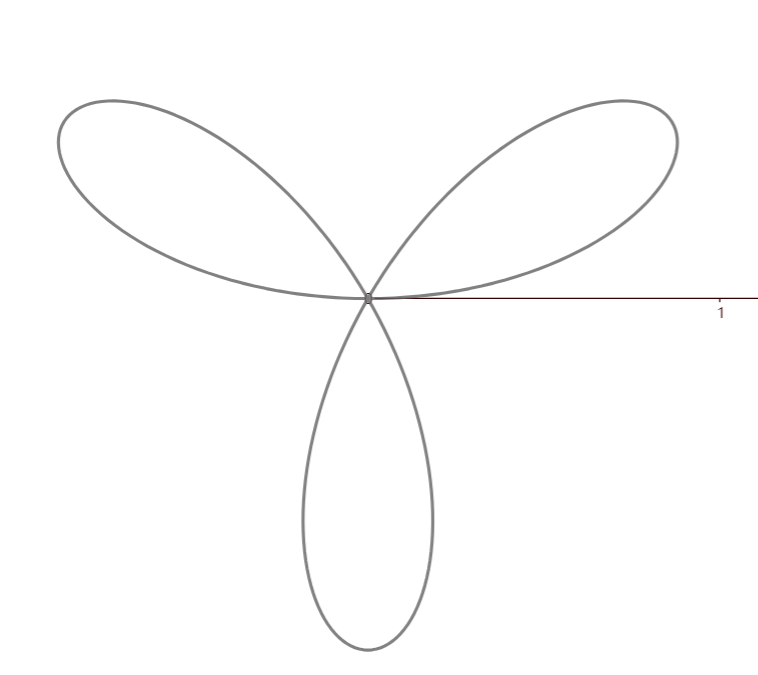
\includegraphics[width=0.45\textwidth]{"figure/Summary/三叶玫瑰线2.png"}}
	\subfigure[伯努利双扭线$\rho^2=a^2\cos 2\theta$]{
	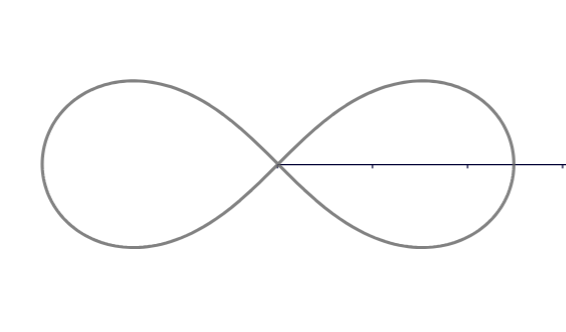
\includegraphics[width=0.45\textwidth]{"figure/Summary/伯努利双扭线.png"}}
	\caption{曲线图形}
\end{figure}

\section{两类欧拉积分}

\begin{definition}[$Gamma$ 函数和 $Beta$函数]	
	1. $Gamma$ 函数(欧拉第一类积分)
	$$B(p,q)=\int_{0}^{1}x^{p-1}(1-x)^{q-1}dx=B(q,p)$$
	
	我们有:  $$B(a,b)=(\frac{x^a(1-x)^b}{a})|_{0}^{1}+\frac{b-1}{a}\int_{0}^{1}x^{a}(1-x)^{b-2}dx$$
	$$B(a,b)=\frac{b-1}{a}\int_{0}^{1}(x-1+1)x^{a-1}(1-x)^{b-2}$$
	$$\mathcolorbox{yellow}{B(a,b)=\frac{b-1}{a}[B(a,b-1)-B(a,b)]}$$ $$\mathcolorbox{yellow}{B(a,b)=\frac{b-1}{a+b-1}B(a,b-1)}$$
	
	特别的,我们有:  $$\mathcolorbox{yellow}{B(m,n)=\frac{(n-1)!(m-1)!}{(m+n-1)!}}$$
	
	2.$Beta$函数(第二类欧拉积分)
	$$\Gamma(\alpha)=\int_{0}^{+\infty}x^{\alpha-1}e^{-x}dx$$
	
	我们有:  $$\Gamma(\alpha)=(-x^{\alpha-1}e^{-x})|_{0}^{+\infty}+(\alpha-1)\int_{0}^{+\infty}x^{\alpha-2}e^{-x}dx$$
	$$\mathcolorbox{red}{\Gamma(\alpha)=(\alpha-1)\Gamma(\alpha-1)},\alpha>1$$
	
	特别的,我们有:  $$\mathcolorbox{red}{\Gamma(n+1)=n!}$$
	
	3. 两类积分之间的关系
	
	转换公式:  
	$$B(a,b)=\frac{\Gamma(a)\Gamma(b)}{\Gamma(a+b)}$$
	
\end{definition}
10. 常用极限技巧
\begin{theorem}\label{the: 常用极限技巧}
	(i).$\lim\limits_{n\rightarrow +\infty}\sqrt[n]{u_{1}^{n}+u_{2}^{n}+u_{3}^{n}+\cdots+u_{m}^{n}}=\text{max}\{ u_{1},u_{2},\cdots,u_{m}\}$
	
	证明:  $$\text{max}\{ u_{1},u_{2},\cdots,u_{m}\}\leq u_{1}^{n}+u_{2}^{n}+u_{3}^{n}+\cdots+u_{m}^{n}\leq m*\text{max}\{ u_{1},u_{2},\cdots,u_{m}\}$$
	我们将$\text{max}\{ u_{1},u_{2},\cdots,u_{m}\}$记作$a$,$m*\text{max}\{ u_{1},u_{2},\cdots,u_{m}\}$记作$b$,我们利用夹逼准则:  
	$$\lim\limits_{n\rightarrow +\infty}\sqrt[n]{a}=\lim\limits_{n\rightarrow +\infty}\sqrt[n]{b}=\text{max}\{ u_{1},u_{2},\cdots,u_{m}\}$$
\end{theorem}
11.变上限积分奇偶性、周期性和原函数关系
\begin{lemma}\label{lem: 变上限积分奇偶性和周期性与原函数关系}
	$f(x)$连续,$f(x)$与$\int_{a}^{x} f(t)dt$之间的关系
	
	(1).如果$f(x)$是奇函数,$\int_{a}^{x}f(t)dt$是偶函数
	
	(2).如果$f(x)$是偶函数,$\int_{a}^{x}f(t)dt$是奇函数当且仅当$a=0$时成立.
	
	(3).如果 $f(x)$ 是周期函数,$\int_{a}^{x}f(t)dt\text{是周期函数与}\int_{0}^{T}f(t)dt=0\text{等价}$
	
	\begin{eqnarray*}
		&&\text{证明:  我们令} F(x)=\int_{a}^{x}f(t)dt\\
		&&(i).\text{必要性:  } F(x+T)-F(x)=\int_{x}^{x+T}f(t)dt=\int_{0}^{T}f(t)dt=0\\
		&&(ii).\text{充分性:  }
		\int_{0}^{T}f(t)dt=0\Leftrightarrow F(x+T)-F(x)=0
	\end{eqnarray*}
\end{lemma}
12. 阿达玛不等式
\begin{figure}[htbp]
	\centering
	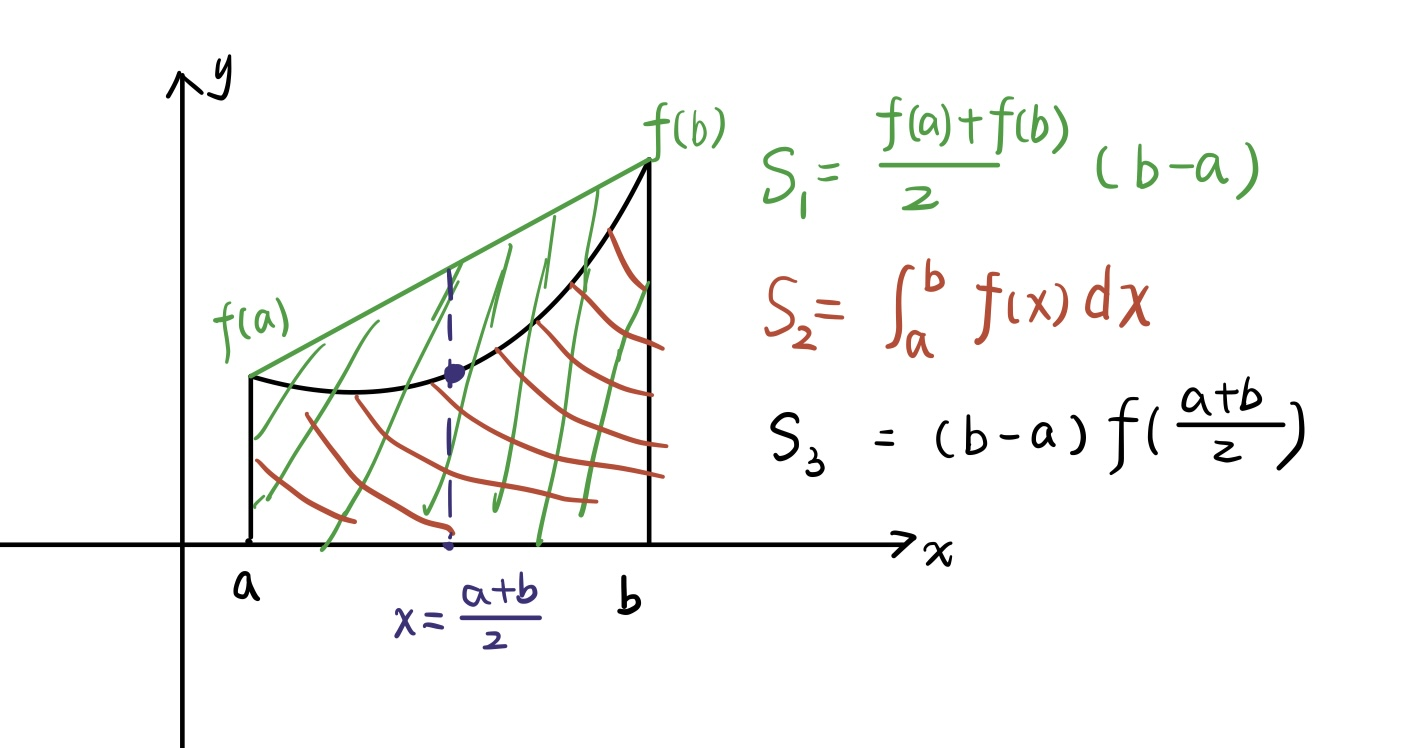
\includegraphics[width=15cm,height=8cm]{"figure/Summary/阿达玛不等式.jpg"}
	\caption{$Hadamard$不等式}
	\label{Figure: $Hadamard$不等式}
\end{figure} 
\begin{theorem}[$Hadamard$不等式]\label{thm: $Hadamard$不等式}
	$f(x)$在$[a,b]$上具有二阶导数,且$f''(x)\geq 0$,下面不等式成立:  
	$$f(\dfrac{a+b}{2})\leq \dfrac{1}{b-a}\int_{a}^{b}f(t)dt\leq \dfrac{1}{2}[f(a)+f(b)]$$
	\begin{proof}
		
		原不等式可以化为:  
		$$(b-a)f(\dfrac{a+b}{2})\leq\int_{a}^{b}f(t)dt\leq\dfrac{b-a}{2}[f(a)+f(b)]$$
		
		我们由图\ref{Figure: $Hadamard$不等式}可以发现:  
		
		不等式左边表示的过$(\dfrac{a+b}{2},f(\dfrac{a+b}{2}))$的切线与$x=a,x=b,y=0$围成的图形的面积$S_{3}$;
		
		不等式中间表示的是$f(x)$与$x=a,x=b,y=0$围成的曲边梯形的面积$S_{2}$;
		
		不等式右边表示的是直线$x=a,x=b,y=0$与直线$y=\dfrac{f(b)-f(a)}{b-a}(x-a)+f(a)$围成的梯形的面积$S_{1}$.
		
		我们可以由图形上直观的看出三个面积的大小关系:  $S_{3}\leq S_{2}\leq S_{1}$
		
		对于左边的不等式,我们将$f(x)$在$x=\dfrac{a+b}{2}$处展开得到:  
		$$f(x)=f(\dfrac{a+b}{2})+f'(\dfrac{a+b}{2})(x-\dfrac{a+b}{2})+f''(\xi)(x-\dfrac{a+b}{2})^2$$
		
		我们由$f''(x)>0$,我们可以得到:  
		$$f(x)>f(\dfrac{a+b}{2})+f'(\dfrac{a+b}{2})(x-\dfrac{a+b}{2})$$
		
		两边同时在$[a,b]$内取定积分得到:  
		$$\int_{a}^{b}f(x)dx>\int_{a}^{b}[f(\dfrac{a+b}{2})+f'(\dfrac{a+b}{2})(x-\dfrac{a+b}{2})]=(b-a)f(\dfrac{a+b}{2})$$
		
		对于右边的不等式,我们构造辅助函数:  
		$$F(x)=\dfrac{x-a}{2}[f(x)+f(a)]-\int_{a}^{x}f(t)dt,\ F(a)=0$$
		$$\left\lbrace
		\begin{array}{l}
			F'(x)=\dfrac{x-a}{2}f'(x)-\dfrac{f(x)-f(a)}{2}\\
			F''(x)=\dfrac{x-a}{2}f''(x)
		\end{array}
		\right. F'(0)=0,F''(x)\geq 0\Rightarrow F'(x)\geq 0$$
		
		我们得到$F'(x)\geq 0\Rightarrow F(x)\text{单调递增}$,$F(x)\geq F(a)=0$
	\end{proof}
\end{theorem}
13.$\lim\limits_{n\rightarrow +\infty}\dfrac{x_{n+1}}{x_{n}}\text{相关命题}$
\begin{theorem}[极限推论]
	1. $\lim\limits_{n\rightarrow +\infty}x_{n}=a$
	
	(i). $a\neq 0\Rightarrow \lim\limits_{n\rightarrow +\infty}\dfrac{x_{n+1}}{x_{n}}=1$
	
	(ii). $a=0\Rightarrow \lim\limits_{n\rightarrow +\infty}\dfrac{x_{n+1}}{x_{n}} \text{不一定存在}$
	
	2. $\lim\limits_{n\rightarrow +\infty}\dfrac{x_{n+1}}{x_{n}}=a$
	
	$$\left\lbrace 
	\begin{array}{l}
		\lim\limits_{n\rightarrow +\infty}x_{n}=\infty \text{当}|a|>1\\
		\lim\limits_{n\rightarrow +\infty}x_{n}=0,\text{当}|a|<1\\
		\lim\limits_{n\rightarrow +\infty}x_{n}\text{不确定},\text{当}|a|=1
	\end{array}
	\right. $$
	
	3. $\lim\limits_{n\rightarrow +\infty}\dfrac{x_{n+1}}{x_{n}}\text{存在且}x_{n}>0$,我们有:  
	$$\lim\limits_{n\rightarrow +\infty}\sqrt[n]{x_{n}}=\lim\limits_{n\rightarrow +\infty}\dfrac{x_{n+1}}{x_{n}}$$
\end{theorem}


\section{谱分解定理}

\begin{definition}[代数重复度]
	设$\lambda_{1},\lambda_{2},\cdots,\lambda_{k}$是矩阵$A\in \mathbb{C}^{n\times n}$的相异特征值,其重数分别为$r_{1},r_{2},\cdots,r_{k}$,称$r_{i}$为矩阵$A$的特征值$\lambda_{i}$的代数重复度.
\end{definition}
\begin{definition}[几何重复度]
	齐次方程组$Ax=\lambda_{i}x\ (i=1,2,\cdots,k)$的解空间$V_{\lambda_{i}}$称为$A$的对应于特征值$\lambda_{i}$的特征空间,则$V_{\lambda_{i}}$的维数称为$A$的特征值$\lambda_{i}$的几何重复度.
\end{definition}
\begin{definition}[单纯矩阵]
	若矩阵$A$的每一个特征值的代数重复度与几何重复度相等,则称矩阵$A$为单纯矩阵.
\end{definition}
\begin{definition}[幂等矩阵]
	若$A$为方阵,且$A^2=A$,则称$A$为幂等矩阵.
\end{definition}
\begin{property}[幂等矩阵$A$性质]
	\begin{itemize}
		\item (1). $A$是单纯矩阵,且其$Jordan$标准型为$\left(\begin{matrix}
			I_{r}&0\\0&0
		\end{matrix} \right) $
		\item (2). $A$的特征值只能为$0$或者$1$
		\item (3). $rank(A)=tr(A)$
		\item (4). $Ax=x\Leftrightarrow x\in\mathbb{R}(A)$
		\item (5). $A$一定可以相似对角化
	\end{itemize}
\end{property}
\begin{theorem}[谱分解定理]\label{the: 谱分解定理}
	设$A\in\mathbb{C}^{n\times n}$是单纯矩阵,矩阵$A$有$k$个相异特征值$\lambda_{i}\ (i=1,2,\cdots,k)$,$\exists A_{i}\in \mathbb{C}^{n\times n}\ (i=1,2,\cdots,k)$,使得
	$$A=\sum\limits_{i=1}^{k}\lambda_{i}G_{i}$$
	
	此式称为矩阵$A$的谱分解,$G_{1},G_{2},\cdots,G_{k}$称为$A$的族谱,且满足一下性质:  
	\begin{property}[谱分解谱族$G_{i}$性质]
		\begin{itemize}
			\item (1). 幂等性:  $G_{i}^2=G_{i}$
			\item (2). 分离性:  $G_{i}G_{j}=0\ (i\neq j)$
			\item (3). 可加性:  $\sum\limits_{i=1}^{k}G_{i}=E_{n}$
		\end{itemize}
	\end{property}
	\begin{corollary}[谱族$G_{i}$推论]
		\begin{itemize}
			\item $AG_{i}=G_{i}A=\lambda_{i}G_{i}$
			\item $rank(G_{i})=m_{i}$
			\item $G_{i}$是唯一的,$G$的族谱是唯一的.
		\end{itemize}
	\end{corollary}
	\begin{proposition}
		矩阵$A$是单纯矩阵等价为存在$k$个矩阵$G_{i},\ (i=1,2,\cdots,k)$满足:  
		\begin{itemize}
			\item (1). $G_{i}G_{j}=\left\lbrace
			\begin{array}{l}
				G_{i},\ i=j\\0,\ i\neq j
			\end{array}
			\right. $
			\item (2). $\sum\limits_{i=1}^{k}G_{i}=E_{n}$
			\item (3). $A=\sum\limits_{i=1}^{k}\lambda_{i}G_{i}$
			\item (4). $f(A)$为任意多项式,则$$f(A)=\sum\limits_{i=1}^{k}f(\lambda_{i})G_{i}$$
			\item (5). $A^m=\sum\limits_{i=1}^{k}\lambda_{i}^mG_{i}$
		\end{itemize}
	\end{proposition}
\end{theorem}
\begin{anymark}[证明]
	1. 必要性
	 
	(1). 当$k=n$时:  
	
	我们由$A$是单纯矩阵可以得到矩阵$A$可以相似对角化
	$$A=P\Lambda P^{-1},\text{其中}\Lambda=diag\{\lambda_{1},\lambda_{2},\cdots,\lambda_{n}\}$$
	
	我们不妨设$P=(v_{1},v_{2},\cdots,v_{n})$,$P^{-1}=\left( \begin{matrix}
		\omega_{1}^{T}\\\omega_{2}^{T}\\ \vdots\\\omega_{n}^{T}
	\end{matrix}\right) $,我们可以得到:  
	$$A=(v_{1},v_{2},\cdots,v_{n})\left[\begin{matrix}
		\lambda_{1}&0&\cdots&0\\
		0&\lambda_{2}&\cdots&0\\
		\cdots&\cdots&\cdots&\cdots\\
		0&0&\cdots&\lambda_{n}
	\end{matrix} \right] \left( \begin{matrix}
		\omega_{1}^{T}\\\omega_{2}^{T}\\ \vdots\\\omega_{n}^{T}
	\end{matrix}\right) \Rightarrow A=\sum\limits_{i=1}^{n}\lambda_{i}v_{i}\omega_{i}^{T}=\sum\limits_{i=1}^{n}\lambda_{i}G_{i},\ \text{其中}G_{i}=v_{i}\omega_{i}^{T}$$
	
	我们由$\left\lbrace
	\begin{array}{l}
		P^{-1}P=E_{n}\\
		PP^{-1}=E_{n}
	\end{array}
	\right.\Rightarrow\left\lbrace
	\begin{array}{l}
		\omega_{i}^{T}v_{j}=\left\lbrace
		\begin{array}{l}
			1,\ i=j\\
			0,\ i\neq j
		\end{array}
		\right. \\
		\sum\limits_{i=1}^{n}v_{i}\omega_{i}^{T}=\sum\limits_{i=1}^{n}G_{i}=E_{n}
	\end{array}
	\right.$
	
	对于任意$i,j\in(1,n),G_{i}G_{j}=v_{i}(\omega_{i}^{T}v_{j})\omega_{j}^{T}$,我们可以得到:  
	$$G_{i}G_{j}=\left\lbrace
	\begin{array}{l}
		v_{i}\omega_{i}^{T}=G_{i},\ i=j\\
		0,\ i\neq j
	\end{array}
	\right. \Rightarrow A_{i}\text{是幂等矩阵}$$
	
	(2). 当$k<n$时:  
	
	我们由矩阵$A$是单纯矩阵,可以得到:  $A=P\Lambda P^{-1}$
	$$\left\lbrace
	\begin{array}{l}
		P=(v_{11},v_{12},\cdots,v_{1r_{1}},v_{21},v_{22},\cdots,v_{2r_{2}},\cdots,v_{k1},v_{k2},\cdots,v_{kr_{k}})\\
		P^{-1}=(\omega_{11}^{T},\omega_{12}^{T},\cdots,\omega_{1r_{1}}^{T},\omega_{21}^{T},\omega_{22}^{T},\cdots,\omega_{2r_{2}}^{T},\cdots,\omega_{k1}^{T},\omega_{k2}^{T},\cdots,\omega_{kr_{k}}^{T})^{T}
	\end{array}
	\right. $$
	$$A=\sum\limits_{i=1}^{k}\lambda_{i}\sum\limits_{j=1}^{r_{i}}B_{ij}\stackrel{G_{i}=\sum\limits_{j=1}^{r_{i}}B_{ij}}{\longrightarrow}A=\sum\limits_{i=1}^{k}\lambda_{i}G_{i}$$
	$$P^{-1}P=E_{n}\Rightarrow \omega_{ij}^{T}v_{lk}=\left\lbrace
	\begin{array}{l}
		1,\ i=l,j=k\\
		0,\ i\neq l\text{或}j\neq k
	\end{array}
	\right. $$
	$$B_{ij}B_{lk}=v_{ij}(\omega_{ij}^{T}v_{lk})\omega_{lk}^{T}=\left\lbrace
	\begin{array}{l}
		B_{ij},\ i=l,j=k\\
		0,\ i\neq l\text{或}j\neq k
	\end{array}
	\right. \Rightarrow G_{i}G_{j}=\sum\limits_{p=1}^{r_{i}}B_{ip}\sum\limits_{q=1}^{r_{j}}B_{jq}=\left\lbrace
	\begin{array}{l}
		G_{i},\ i=j\\0,\ i\neq j
	\end{array}
	\right. $$
	$$\sum\limits_{i=1}^{k}G_{i}=\sum\limits_{i=1}^{n}B_{i}=E_{n}$$
	(2). 充分性
	
	我们首先可以得到矩阵$G_{i}$均为幂等矩阵,我们不妨设$dim\mathbb{R}(G_{i})=n_{i}$,我们可以得到:  
	$$n_{i}=tr(G_{i})\Rightarrow \sum\limits_{i=1}^{k}n_{i}=\sum\limits_{i=1}^{k}tr(G_{i})=tr(\sum\limits_{i=1}^{k}G_{i})=tr(E_{n})=n$$
	
	我们取$X_{i}$为$\mathbb{R}(G_{i})$的基列构成的阵,则$X=(X_{1},X_{2},\cdots,X_{k})$是$n\times n$矩阵,且$G_{i}$的列向量都可以由$X_{i}$线性表出,我们可以得到:  
	$$G_{i}=(X_{i}\beta_{1},X_{i}\beta_{2},\cdots,X_{i}\beta_{n})=X_{i}Y_{i}$$
	$$XY=(X_{1},X_{2},\cdots,X_{n})\left( \begin{matrix}
		Y_{1}\\Y_{2}\\\vdots\\Y_{n}
	\end{matrix}\right)=\sum\limits_{i=1}^{n}X_{i}Y_{i}=E_{n}\Rightarrow \text{矩阵}X\text{可逆}$$

	$$YX=\left( \begin{matrix}
		Y_{1}\\Y_{2}\\\vdots\\Y_{n}
	\end{matrix}\right)(X_{1},X_{2},\cdots,X_{k})=\left[ \begin{matrix}
	Y_{1}\\Y_{2}\\\cdots\\Y_{k}
\end{matrix}\right] =\left[\begin{matrix}
Y_{1}X_{1}&Y_{1}X_{2}&\cdots&Y_{1}X_{k}\\
Y_{2}X_{1}&Y_{2}X_{2}&\cdots&Y_{2}X_{k}\\
\cdots&\cdots&\cdots&\cdots\\
Y_{k}X_{1}&Y_{k}X_{2}&\cdots&Y_{k}X_{k}\\
\end{matrix} \right] =E_{n}=\left[\begin{matrix}
E_{r_{1}}&0&\cdots&0\\
0&E_{r_{2}}&\cdots&0\\
\cdots&\cdots&\cdots&\cdots\\
0&0&\cdots&E_{r_{k}}\\
\end{matrix} \right]$$

我们可以得到:  
$$Y_{i}X_{j}=\left\lbrace
\begin{array}{l}
	E_{r_{i}},\ i=j\\
	0,\ i\neq j
\end{array}
\right. \Rightarrow G_{i}X_{j}=x_{i}Y_{i}X_{j}=\left\lbrace
\begin{array}{l}
	X_{i},\ i=j\\
	0,\ i\neq j
\end{array}
\right. $$

	我们利用幂等矩阵的性质
	\begin{eqnarray*}
		AX&=&(\sum\limits_{i=1}^{k}\lambda_{i}G_{i})(X_{1},X_{2},\cdots,X_{k})\\
		&=&((\sum\limits_{i=1}^{k}\lambda_{i}G_{i})X_{1},(\sum\limits_{i=1}^{k}\lambda_{i}G_{i})X_{2},\cdots,(\sum\limits_{i=1}^{k}\lambda_{i}G_{i})X_{k})\\
		&=&(\lambda_{1}X_{1},\lambda_{2}X_{2},\cdots,\lambda_{k}X_{k})\\
		&=&(X_{1},X_{2},\cdots,X_{k})\left[\begin{matrix}
			E_{r_{1}}&0&\cdots&0\\
			0&E_{r_{2}}&\cdots&0\\
			\cdots&\cdots&\cdots&\cdots\\
			0&0&\cdots&E_{r_{k}}\\
		\end{matrix} \right]\\
	&=&X\Lambda\Rightarrow A=X\Lambda X^{-1} 
	\end{eqnarray*}
	
	(3). 谱分解唯一性
	
	我们不妨假设$F_{1},F_{2},\cdots,F_{k}$满足:  
	$$\left\lbrace
	\begin{array}{l}
		F_{i}F_{j}=0,\ i\neq j\\
		F_{i}^2=F_{i}\\
		A=\sum\limits_{i=1}^{k}\lambda_{i}F_{i}\\
		\sum\limits_{i=1}^{k}F_{i}=E_{n}
	\end{array}
	\right. $$
	
	我们由族谱$G_{i}$性质推论可以得到:  
	$$\left\lbrace
	\begin{array}{l}
		AG_{i}=G_{i}A=\lambda_{i}G_{i}\\
		AF_{i}=F_{i}A=\lambda_{i}F_{i}
	\end{array}
	\right. \Rightarrow \left\lbrace
	\begin{array}{l}
		AG_{i}F_{j}=\lambda_{i}G_{i}F_{j}\\
		\lambda_{i}G_{i}F_{j}=G_{i}AF_{j}\\
		G_{i}AF_{j}=\lambda_{j}G_{i}F_{j}
	\end{array}
	\right. \Rightarrow G_{i}F_{j}=0,\ i\neq j$$
	
	我们得到:  $$G_{i}=G_{i}E_{n}=G_{i}(\sum\limits_{j=1}^{k}F_{j})=G_{i}F_{i}=(\sum\limits_{j=1}^{k}G_{j})F_{i}=F_{i}$$
	
	综上所述,矩阵$A$的谱分解是唯一的.
\end{anymark}
\myspace{1}

\section{积分训练}
40. 积分训练
\begin{anymark}[积分训练]
	(1). $\int \dfrac{x\sin x}{(1+\cos^2x)^{\frac{3}{2}}}dx$
	\myspace{1}
	\begin{solution}
		
		我们令$f(x)=\dfrac{\sin x}{(1+\cos^2x)^{\frac{3}{2}}}$
		\begin{eqnarray*}
			F(x)&=&\int f(x)dx\\
				&=&\int -\dfrac{d\cos x}{(1+\cos^2x)^{\frac{3}{2}}}\\
				&=&\int -\dfrac{du}{(1+u^2)^{\frac{3}{2}}}\\
				&\xlongequal{u=\tan t}&\int (-\cos t)dt\\
				&=&-\sin t+C\\
				&\xlongequal{\sin t=\frac{u}{\sqrt{1+u^2}}}&-\dfrac{\cos x}{\sqrt{1+\cos^2 x}}+C
		\end{eqnarray*}
		
		原不定积分等价于:  
		\begin{eqnarray*}
			I&=&\int xd(F(x))\\
			&=&xF(x)-\int F(x)dx\\
			&=&-\dfrac{x\cos x}{\sqrt{1+\cos^2 x}}+\int \dfrac{\cos x}{\sqrt{1+\cos^2 x}}dx\\
			&=&-\dfrac{x\cos x}{\sqrt{1+\cos^2 x}}+\int \dfrac{d\sin x}{\sqrt{2-\sin^2 x}}\\
			&=&\arcsin(\dfrac{\sin x}{\sqrt{2}})-\dfrac{x\cos x}{\sqrt{1+\cos^2 x}}+C
		\end{eqnarray*}
	\end{solution}
	\myspace{1}
	(2). $\int \dfrac{x^3\arccos x}{\sqrt{1-x^2}}dx$
	\myspace{1}
	\begin{solution}
		
		我们令$f(x)=\dfrac{\arccos x}{\sqrt{1-x^2}}$
		\begin{eqnarray*}
			F(x)&=&\int f(x)dx\\
			&=&\int -\arccos xd(\arccos x)\\
			&=&-\dfrac{1}{2}(\arccos x)^2+C
		\end{eqnarray*}
		
		原不定积分等价于:  
		\begin{eqnarray*}
			I&=&\int x^3d(F(x))\\
			&=&x^3F(x)-\int F(x)dx\\
			&=&-\dfrac{x^3}{2}(\arccos x)^2-\dfrac{1}{2}\int (\arccos x)^2dx\\
			&\xlongequal[x=\cos u]{u=\arccos x}&-\dfrac{x^3}{2}(\arccos x)^2+\dfrac{1}{2}\int u^2\sin udu\\
			&\xlongequal{\text{分部积分}}&-\dfrac{x^3}{2}(\arccos x)^2-\dfrac{u^2}{2}\cos u+u\sin u+\cos u+C\\
			&\xlongequal[\sin u=\sqrt{1-x^2}]{u=\arccos x}&-\dfrac{x^3}{2}(\arccos x)^2-\dfrac{x(\arccos x)^2}{2}+\sqrt{1-x^2}\arccos x+x+C
		\end{eqnarray*}
	\end{solution}
	\myspace{1}
	(3). $\int \dfrac{x+\sin x\cos x}{(x\sin x+\cos x)^2}dx$
	\myspace{1}
	\begin{solution}
		
		原不定积分等价于:  
		\begin{eqnarray*}
			I&=&\int \dfrac{xd\tan x+\tan xdx}{(x\tan x+1)^2}\\
			&=&\int \dfrac{dx\tan x}{(x\tan x+1)^2}\\
			&=&-\dfrac{1}{x\tan x+1}+C
		\end{eqnarray*}
	\end{solution}
	\myspace{1}
	(4). $\int \dfrac{1-ln x}{(x-ln x)^2}dx$
	\myspace{1}
	\begin{solution}
		
		我们令:  $f(x)=\dfrac{h(x)}{x-ln x}$
		\begin{eqnarray*}
			f'(x)&=&\dfrac{h'(x)(x-lnx)-h(x)(1-\dfrac{1}{x})}{(x-ln x)^2}\\
			&=&\dfrac{1-ln x}{(x-ln x)^2}
		\end{eqnarray*}
	
	当$h(x)=x$时,$f'(x)=\dfrac{1-ln x}{(x-ln x)^2}$,原不定积分为:  $I=\dfrac{x}{x-ln x}+C$
	\end{solution}
	\myspace{1}
	(5). $\int \dfrac{x\cos x}{(x+\cos x)^2}dx$
	\myspace{1}
	\begin{solution}
		
		我们令:  $f(x)=\dfrac{h(x)}{x+\cos x}$
		\begin{eqnarray*}
			f'(x)&=&\dfrac{h'(x)(x+\cos x)-h(x)(1-\sin x)}{(x+\cos x)^2}\\
			&=&\dfrac{x\cos x}{(x+\cos x)^2}
		\end{eqnarray*}
		
		当$h(x)=\sin x+1$时,$f'(x)=\dfrac{x\cos x}{(x+\cos x)^2}$,原不定积分为:  $I=\dfrac{\sin x+1}{x+\cos x}+C$
	\end{solution}
	\myspace{1}
	(6). $\int \dfrac{\cos^2x-x^2\sin x}{(x+\cos x)^2}dx$
	\myspace{1}
	\begin{solution}
		
		我们令:  $f(x)=\dfrac{h(x)}{x+\cos x}$
		\begin{eqnarray*}
			f'(x)&=&\dfrac{h'(x)(x+\cos x)-h(x)(1-\sin x)}{(x+\cos x)^2}\\
			&=&\dfrac{\cos^2x-x^2\sin x}{(x+\cos x)^2}
		\end{eqnarray*}
		
		当$h(x)=x\cos x$时,$f'(x)=\dfrac{x\cos x}{(x+\cos x)^2}$,原不定积分为:  $I=\dfrac{x\cos x}{x+\cos x}+C$
	\end{solution}
	\myspace{1}
	(7). $\int \dfrac{x\sin x+\cos x}{x^2+\cos^2x}dx$
	\myspace{1}
	\begin{solution}
		
		原不定积分等价为:  
		\begin{eqnarray*}
			I&=&\int \dfrac{\frac{x\sin x+\cos x}{x^2}}{1+\left( \frac{\cos x}{x}\right)^2}dx\\
			&=&-\int \dfrac{d\frac{\cos x}{x}}{1+\left( \frac{\cos x}{x}\right)^2}\\
			&=&-\arctan(\dfrac{\cos x}{x})+C
		\end{eqnarray*}
	
		原不定积分为:  $I=-\arctan(\dfrac{\cos x}{x})+C$
	\end{solution}
	\myspace{1}
	(8). $\int \dfrac{e^x(x-1)}{x^2+e^{2x}}dx$
	\myspace{1}
	\begin{solution}
		
		原不定积分等价为:  
		\begin{eqnarray*}
			I&=&\dfrac{\frac{e^x(x-1)}{x^2}}{1+\left(\frac{e^x}{x}\right)^2}dx\\
			&=&-\int \dfrac{d\frac{e^x}{x}}{1+\left( \frac{e^x}{x}\right)^2}\\
			&=&-\arctan(\dfrac{e^x}{x})+C
		\end{eqnarray*}
		
		原不定积分为:  $I=-\arctan(\dfrac{e^x}{x})+C$
	\end{solution}
	\myspace{1}
	(9). $\int e^{\sec x}(\tan x-\sin x)dx$
	\myspace{1}
	\begin{solution}
		
		我们令:  $f(x)=h(x)e^{\sec x}$
		\begin{eqnarray*}
			f'(x)&=&h'(x)e^{\sec x}+h(x)e^{\sec x}\dfrac{\sin x}{\cos^2x}\\
			&=&\dfrac{h'(x)\cos^2x+h(x)\sin x}{\cos^2x}e^{\sec x}\\
			&=&(\tan x-\sin x)e^{\sec x}
		\end{eqnarray*}
		
		当$h(x)=\cos x$时,$f'(x)=(\tan x-\sin x)e^{\sec x}$,原不定积分为:  $I=\cos xe^{\sec x}+C$
	\end{solution}
	\myspace{1}
	(10). $\int e^{\frac{1}{x}}(2x-1)dx$
	\myspace{1}
	\begin{solution}
		
		我们令:  $f(x)=h(x)e^{\frac{1}{x}}$
		\begin{eqnarray*}
			f'(x)&=&h'(x)e^{\frac{1}{x}}-h(x)e^{\sec x}\dfrac{1}{x^2}\\
			&=&\dfrac{h'(x)x^2-h(x)}{x^2}e^{\sec x}\\
			&=&(2x-1)e^{\frac{1}{x}}
		\end{eqnarray*}
		
		当$h(x)=x^2$时,$f'(x)=(2x-1)e^{\frac{1}{x}}$,原不定积分为:  $I=x^2e^{\frac{1}{x}}+C$
	\end{solution}
	\myspace{1}
	(11). $\int e^{\sin x}\dfrac{x\cos^3 x-\sin x}{\cos^2x}dx$
	\myspace{1}
	\begin{solution}
		
		我们令:  $f(x)=h(x)\dfrac{e^{\sin x}}{\cos x}$
		\begin{eqnarray*}
			f'(x)&=&\dfrac{\left[h(x)e^{\sin x}\cos x+h'(x)e^{\sin x}\right]\cos x+h(x)e^{\sin x}\sin x }{\cos^2 x}\\
			&=&\dfrac{e^{\sin x}}{\cos^2 x}\left[ h(x)\cos^2 x+h'(x)\cos x+h(x)\sin x\right] \\
			&=&e^{\sin x}\dfrac{x\cos^3 x-\sin x}{\cos^2x}
		\end{eqnarray*}
		
		当$h(x)=x\cos x-1$时,$f'(x)=e^{\sin x}\dfrac{x\cos^3 x-\sin x}{\cos^2x}$,原不定积分为:  $I=\dfrac{(x\cos x-1)e^{\sin x}}{\cos x}+C$
	\end{solution}
	\myspace{1}
	(12). $\int e^{x^3}(10x-9x^7)dx$
	\myspace{1}
	\begin{solution}
		
		我们令:  $f(x)=h(x)e^{x^3}$
		\begin{eqnarray*}
			f'(x)&=&e^{x^3}\left(h'(x)+3x^2h(x)\right) \\
			&=&e^{x^3}(10x-9x^7)
		\end{eqnarray*}
		
		当$h(x)=5x^2-3x^5$时,$f'(x)=e^{x^3}(10x-9x^7)$,原不定积分为:  $I=e^{x^3}(5x^2-3x^5)+C$
	\end{solution}
	\myspace{1}
	(13). $\int \dfrac{1}{x\sqrt{x-1}}dx$
	\myspace{1}
	\begin{solution}
		
		原不定积分等价于:  
		\begin{eqnarray*}
			I&\xlongequal[x=u^2+1]{u=\sqrt{x-1}}&\int \dfrac{2u}{(u^2+1)u}du\\
			&=&2\arctan u+C\\
			&=&2\arctan \sqrt{x-1}+C
		\end{eqnarray*}
	
	原不定积分为:  $I=2\arctan \sqrt{x-1}+C$
	\end{solution}
	\myspace{1}
	(14). $\int \dfrac{1}{x+\sqrt{x-1}}dx$
	\myspace{1}
	\begin{solution}
		
		原不定积分等价于:  
		\begin{eqnarray*}
			I&\xlongequal[x=u^2+1]{u=\sqrt{x-1}}&\int \dfrac{2u}{(u^2+1)+u}du\\
			&=&\int \dfrac{2u}{u^2+u+1}du-\int \dfrac{1}{\frac{3}{4}+(u+\frac{1}{2})^2}du\\
			&=&ln(u^2+u+1)-\frac{2}{\sqrt{3}}\arctan\dfrac{2u+1}{\sqrt{3}}+C\\
			&=&ln(x+\sqrt{x-1})-\dfrac{2}{\sqrt{3}}\arctan\dfrac{2\sqrt{x-1}+1}{\sqrt{3}}+C
		\end{eqnarray*}
		
		原不定积分为:  $I=ln(x+\sqrt{x-1})-\dfrac{2}{\sqrt{3}}\arctan\dfrac{2\sqrt{x-1}+1}{\sqrt{3}}+C$
	\end{solution}
	\myspace{1}
	(15). $\int \dfrac{1}{x^2\sqrt{2x-1}}dx$
	\myspace{1}
	\begin{solution}
		
		原不定积分等价于:  
		\begin{eqnarray*}
			I&\xlongequal[x=\frac{u^2+1}{2}]{u=\sqrt{2x-1}}&\int \dfrac{4}{(u^2+1)^2}du\\
			&\xlongequal{u=\tan t}&\int 4\cos^2 tdt\\
			&=&2t+\sin 2t\\
			&=&2t+\dfrac{2\tan t}{1+\tan^2t}\\
			&=&2\arctan u+\dfrac{2u}{1+u^2}\\
			&=&2\arctan\sqrt{2x-1}+\dfrac{\sqrt{2x-1}}{x}+C
		\end{eqnarray*}
		
		原不定积分为:  $I=2\arctan\sqrt{2x-1}+\dfrac{\sqrt{2x-1}}{x}+C$
	\end{solution}
	\myspace{1}
	(16). $\int \dfrac{\sqrt{1-x}}{x^3}dx$
	\myspace{1}
	\begin{solution}
		
		原不定积分等价于:  
		\begin{eqnarray*}
			I&\xlongequal[t=\sqrt{1-x}]{x=1-t^2}&\int \dfrac{2t^2}{(t^2-1)^3}dt\\
			&\xlongequal[t=\sec u]{u=\arccos\left(\dfrac{1}{\sqrt{1-x}}\right)}&\int \dfrac{2\cos^2u}{\sin^5 u}du\\
			&=&\int \dfrac{2}{\sin^5 u}du-\int \dfrac{2}{\sin^3 u}du	
		\end{eqnarray*}
		
		我们有:
		$$\left\lbrace
		\begin{array}{l}
			\int \dfrac{1}{\sin^3 x}dx=\dfrac{1}{4}ln\left(\dfrac{1-\cos x}{1+\cos x} \right)-\dfrac{\cos x}{2\sin^2 x}+C\\
			\int \dfrac{1}{\sin^5 x}dx=\dfrac{3}{16}ln\left(\dfrac{1-\cos x}{1+\cos x} \right)+\dfrac{3\cos^3 x-5\cos x}{8\sin^4x}+C
		\end{array}
		\right. $$
		
		\begin{eqnarray*}
			I&=&\dfrac{3}{8}ln\left(\dfrac{1-\cos u}{1+\cos u} \right)+\dfrac{3\cos^3 u-5\cos u}{4\sin^4u}-\dfrac{1}{2}ln\left(\dfrac{1-\cos u}{1+\cos u} \right)+\dfrac{\cos u}{\sin^2 u}\\
			&=&-\dfrac{1}{8}ln\left(\dfrac{1-\cos u}{1+\cos u} \right)-\dfrac{\cos^3 u+\cos u}{4\sin^4 u}\\
			&=&-\dfrac{1}{8}ln\left(\dfrac{t-1}{t+1} \right)-\dfrac{t^3+t}{4(t^2-1)^2}\\
			&=&-\dfrac{1}{8}ln\left(\dfrac{\sqrt{1-x}-1}{\sqrt{1-x}+1} \right)-\dfrac{(2-x)\sqrt{1-x}}{4x^2}+C
		\end{eqnarray*}
	
		原不定积分为:  $I=-\dfrac{1}{8}ln\left(\dfrac{\sqrt{1-x}-1}{\sqrt{1-x}+1} \right)-\dfrac{(2-x)\sqrt{1-x}}{4x^2}+C$
	\end{solution}
	\myspace{1}
	(17). $\int \dfrac{x}{\sqrt{x+1}+\sqrt{x-1}}dx$
	\myspace{1}
	\begin{solution}
		
		原不定积分等价于:  
		\begin{eqnarray*}
			I&=&\int \dfrac{x(\sqrt{x+1}-\sqrt{x-1})}{2}dx\\
			&=&\int \dfrac{x\sqrt{x+1}}{2}dx-\int \dfrac{x\sqrt{x-1}}{2}dx\\
			&=&I_{1}-I_{2}\\
			I_{1}&\xlongequal[u=\sqrt{x+1}]{x=u^2-1}&\int (u^2-1)u^2du\\
			&=&\dfrac{u^5}{5}-\dfrac{u^3}{3}\\
			I_{2}&\xlongequal[t=\sqrt{x-1}]{x=t^2+1}&\int (t^2+1)t^2dt\\
			&=&\dfrac{t^5}{5}+\dfrac{t^3}{3}\\
			I&=&\dfrac{(x+1)^2\sqrt{x+1}}{5}-\dfrac{(x+1)\sqrt{x+1}}{3}-\dfrac{(x-1)^2\sqrt{x-1}}{5}-\dfrac{(x-1)\sqrt{x-1}}{3}+C
		\end{eqnarray*}
		
		原不定积分为:  $I=\dfrac{(x+1)^2\sqrt{x+1}}{5}-\dfrac{(x+1)\sqrt{x+1}}{3}-\dfrac{(x-1)^2\sqrt{x-1}}{5}-\dfrac{(x-1)\sqrt{x-1}}{3}+C$
	\end{solution}
	\myspace{1}
	(18). $\int \dfrac{1}{\sqrt{1+x}+\sqrt{1-x}+\sqrt{2}}dx$
	\myspace{1}
	\begin{solution}
		
		原不定积分等价于:  
		\begin{eqnarray*}
			I&=&\int \dfrac{\sqrt{1+x}+\sqrt{1-x}-\sqrt{2}}{(\sqrt{1+x}+\sqrt{1-x})^2-2}dx\\
			&=&\int \dfrac{\sqrt{1+x}+\sqrt{1-x}-\sqrt{2}}{2\sqrt{1-x^2}}dx\\
			&=&\int \dfrac{1}{2\sqrt{1-x}}dx+\int \dfrac{1}{2\sqrt{1+x}}dx-\int \dfrac{\sqrt{2}}{2\sqrt{1-x^2}}dx\\
			&=&\sqrt{1+x}-\sqrt{1-x}-\dfrac{\sqrt{2}}{2}\arcsin x+C
		\end{eqnarray*}
		
		原不定积分为:  $I=\sqrt{1+x}-\sqrt{1-x}-\dfrac{\sqrt{2}}{2}\arcsin x+C$
	\end{solution}
	\myspace{1}
	(19). $\int \sqrt{\dfrac{1+x}{1-x}}dx$
	\myspace{1}
	\begin{solution}
		
		原不定积分等价于:  
		\begin{eqnarray*}
			I&\xlongequal[x=\frac{t^2-1}{t^2+1}]{t=\sqrt{\frac{1+x}{1-x}}}&\int\dfrac{4t^2}{(t^2+1)^2}dt\\
			&\xlongequal{t=\tan u}&\int 4\sin^2 udu\\
			&=&2u-\sin2u\\
			&=&2u-\dfrac{2\tan u}{1+\tan^2 u}+C\\
			&=&2\arctan\sqrt{\dfrac{1+x}{1-x}}-\sqrt{1-x^2}+C
		\end{eqnarray*}
		
		原不定积分为:  $I=2\arctan\sqrt{\dfrac{1+x}{1-x}}-\sqrt{1-x^2}+C$
	\end{solution}
	\myspace{1}
	(20). $\int x\sqrt{\dfrac{x}{3-x}}dx$
	\myspace{1}
	\begin{solution}
		
		原不定积分等价于:  
		\begin{eqnarray*}
			I&\xlongequal[x=\frac{3t^2}{t^2+1}]{t=\sqrt{\frac{x}{3-x}}}&\int\dfrac{18t^4}{(t^2+1)^3}dt\\
			&\xlongequal{t=\tan u}&\int 18\sin^4 udu\\
			&=&\int \dfrac{9(1-2\cos 2u+\cos^22u)}{2}du\\
			&=&\int \left( \dfrac{27}{4}+\dfrac{9}{4}\cos 4u-9\cos 2u\right)du\\
			&=&\dfrac{27}{4}u+\dfrac{9}{16}\sin 4u-\dfrac{9}{2}\sin 2u\\
			&\xlongequal[\sin 2u=\frac{2t}{1+t^2}]{\cos 2u=\frac{1-t^2}{1+t^2}}& \dfrac{27}{4}\arctan\sqrt{\dfrac{x}{3-x}}-\dfrac{(9+2x)\sqrt{3x-x^2}}{4}+C
		\end{eqnarray*}
		
		原不定积分为:  $I=\dfrac{27}{4}\arctan\sqrt{\dfrac{x}{3-x}}-\dfrac{(9+2x)\sqrt{3x-x^2}}{4}+C$
	\end{solution}
	\myspace{1}
	(21). $\int \sqrt{\dfrac{x}{1+x}}dx$
	\myspace{1}
	\begin{solution}
		
		原不定积分等价于:  
		\begin{eqnarray*}
			I&\xlongequal[x=\frac{t^2}{1-t^2}]{t=\sqrt{\frac{x}{1+x}}}&\int\dfrac{2t^2}{(t^2-1)^2}dt\\
			&\xlongequal{t=\sec u}&\int \dfrac{2}{\sin^3 u}du\\
			&=&\dfrac{1}{2}ln\left(\dfrac{1-\cos u}{1+\cos u} \right)-\dfrac{\cos u}{\sin^2 u}+C\\
			&=&\dfrac{1}{2}ln\left(\dfrac{t-1}{t+1} \right)-\dfrac{t}{1-t^2}+C\\
			&=&\dfrac{1}{2}ln\left(\dfrac{\sqrt{1+x}-\sqrt{x}}{\sqrt{1+x}+\sqrt{x}} \right)+\sqrt{x+x^2}+C
		\end{eqnarray*}
		
		原不定积分为:  $I=\dfrac{1}{2}ln\left(\dfrac{\sqrt{1+x}-\sqrt{x}}{\sqrt{1+x}+\sqrt{x}} \right)+\sqrt{x+x^2}+C$
	\end{solution}
	\myspace{1}
	(22). $\int \sqrt{\dfrac{x+1}{x-1}}dx$
	\myspace{1}
	\begin{solution}
		
		原不定积分等价于:  
		\begin{eqnarray*}
			I&\xlongequal[x=\frac{t^2+1}{t^2-1}]{t=\sqrt{\frac{x+1}{x-1}}}&\int-\dfrac{4t^2}{(t^2-1)^2}dt\\
			&\xlongequal{t=\sec u}&\int -\dfrac{4}{\sin^3 u}du\\
			&=&ln\left(\dfrac{1+\cos u}{1-\cos u} \right)+\dfrac{2\cos u}{\sin^2 u}+C\\
			&=&ln\left(\dfrac{\sqrt{x+1}+\sqrt{x-1}}{\sqrt{x+1}-\sqrt{x-1}} \right)+\sqrt{x^2-1}+C
		\end{eqnarray*}
		
		原不定积分为:  $I=ln\left(\dfrac{\sqrt{x+1}+\sqrt{x-1}}{\sqrt{x+1}-\sqrt{x-1}} \right)+\sqrt{x^2-1}+C$
	\end{solution}
	\myspace{1}
	(23). $\int \sqrt{x(x+2)}dx$
	\myspace{1}
	\begin{solution}
		
		原不定积分等价于:  
		\begin{eqnarray*}
			I&\xlongequal[x=u-1]{u=x+1}&\int \sqrt{u^2-1}du\\
			&=&\dfrac{u\sqrt{u^2-1}}{2}-\dfrac{ln|u+\sqrt{u^2-1}|}{2}+C\\
			&=&\dfrac{(x+1)\sqrt{x^2+2x}}{2}-\dfrac{ln|x+1+\sqrt{x^2+2x}|}{2}+C
		\end{eqnarray*}
		
		原不定积分为:  $I=\dfrac{(x+1)\sqrt{x^2+2x}}{2}-\dfrac{ln|x+1+\sqrt{x^2+2x}|}{2}+C$
	\end{solution}
	\myspace{1}
	(24). $\int \dfrac{x^2}{\sqrt{-x^2+2x+3}}dx$
	\myspace{1}
	\begin{solution}
		
		原不定积分等价于:  
		\begin{eqnarray*}
			I&\xlongequal[x=2\sin\theta+1]{\sin\theta=\frac{x-1}{2}}&\int (2\sin\theta+1)^2d\theta\\
			&=&3\theta-\sin2\theta-4\cos\theta+C\\
			&=&3\arcsin\dfrac{x-1}{2}-\dfrac{(x+3)\sqrt{-x^2+2x+3}}{2}+C
		\end{eqnarray*}
		
		原不定积分为:  $I=3\arcsin\dfrac{x-1}{2}-\dfrac{(x+3)sqrt{-x^2+2x+3}}{2}+C$
	\end{solution}
	\myspace{1}
	(25). $\int \dfrac{\sin 2x}{\sin^4 x+\cos^4 x}dx$
	\myspace{1}
	\begin{solution}
		
		原不定积分等价于:  
		\begin{eqnarray*}
			I&\xlongequal[x=\arctan u]{\tan x=u}&\int \dfrac{2u}{u^4+1}du\\
			&=&\int \dfrac{1}{(u^2)^2+1}d(u^2)\\
			&=&\arctan u^2+C\\
			&=&\arctan(tan^2 x)+C
		\end{eqnarray*}
		
		原不定积分为:  $I=\arctan(tan^2 x)+C$
	\end{solution}
	\myspace{1}
	(26). $\int \dfrac{e^{\sin x}\sin 2x}{\sin^4(\frac{\pi}{4}+\frac{x}{2})}dx$
	\myspace{1}
	\begin{solution}
		
		原不定积分等价于:  
		\begin{eqnarray*}
			I&=&\int \dfrac{8e^{\sin x}\sin x}{(1+\sin x)^2}d\sin x\\
			&\xlongequal[x=\arcsin u]{\sin x=u}&\int\dfrac{8e^{u}u}{(1+u)^2}du\\
			&=&\dfrac{8e^u}{1+u}+C \\
			&=&\dfrac{8e^{\sin x}}{1+\sin x}+C
		\end{eqnarray*}
		
		原不定积分为:  $I=\dfrac{8e^{\sin x}}{1+\sin x}+C$
	\end{solution}
	\myspace{1}
	(27). $\int \dfrac{1}{\sin^2x+\sin 2x}dx$
	\myspace{1}
	\begin{solution}
		
		原不定积分等价于:  
		\begin{eqnarray*}
			I&=&\int \dfrac{1}{\tan^2 x+2\tan x}d\tan x\\
			&=&\int\dfrac{1}{2}\left(\dfrac{1}{\tan x}-\dfrac{1}{\tan x+2}\right)d\tan x\\
			&=&\dfrac{1}{2}ln|\dfrac{\tan x}{\tan x+2}|+C 
		\end{eqnarray*}
	
	原不定积分为:  $I=\dfrac{1}{2}ln|\dfrac{\tan x}{\tan x+2}|+C $
	\end{solution}
	\myspace{1}
	(28). $\int \dfrac{\sin x}{\cos x+2\sin x}dx$
	\myspace{1}
	\begin{solution}
		
		原不定积分等价于:  $I=\dfrac{A(\cos x+2\sin x)+B(2\cos x-\sin x)}{\cos x+2\sin x}$
		
		我们有:  $\left\lbrace
		\begin{array}{l}
			A+2B=0\\
			2A-B=1
		\end{array}
		\right. \Rightarrow \left\lbrace
		\begin{array}{l}
			A=\dfrac{2}{5}\\
			B=-\dfrac{1}{5}
		\end{array}
		\right. $
		
		原不定积分等价为:  
		\begin{eqnarray*}
			I&=&\dfrac{2}{5}-\dfrac{2\cos x-\sin x}{5(\cos x+2\sin x)}\\
			&=&\dfrac{2x}{5}-\dfrac{ln|\cos x+2\sin x|}{5}+C
		\end{eqnarray*}
	
	原不定积分为:  $I=\dfrac{2x}{5}-\dfrac{ln|\cos x+2\sin x|}{5}+C$
	\end{solution}
	\myspace{1}
\end{anymark}
\myspace{1}


42. 常见不定积分
\begin{anymark}[常见不定积分]
	1. $$\left\lbrace
	\begin{array}{l}
		\int \dfrac{1}{\sin x}dx=ln|\cot x+\csc x|+C\\
		\int \dfrac{1}{\cos x}dx=ln|\tan x+\sec x|+C
	\end{array}
	\right.$$
	\myspace{1}
	2. $$\left\lbrace
	\begin{array}{l}
		\int \dfrac{1}{\sin^2 x}dx=-\cot x+C\\
		\int \dfrac{1}{\cos^2 x}dx=\tan x+C
	\end{array}
	\right.$$
	\myspace{1}
	3. $$\int \dfrac{1}{\sin^3 x}dx$$
	\begin{eqnarray*}
		I&=&-\int \dfrac{1}{\sin^4 x}d\cos x\\
		&=&-\int \dfrac{1}{(1-t^2)^2}dt\\
		&=&\int\left[ \dfrac{A}{t+1}+\dfrac{B}{(t+1)^2}+\dfrac{C}{t-1}+\dfrac{D}{(t-1)^2}\right]dx 
	\end{eqnarray*}
	
	我们令$f(x)=A(t-1)^2(t+1)+B(t-1)^2+C(t+1)^2(t-1)+D(t+1)^2=-1$,我们有:  
	$$\left\lbrace
	\begin{array}{l}
		f(0)=A+B-C+D=-1\\
		f(-1)=4B=-1\\
		f(1)=4D=-1\\
		f(2)=3A+B+9C+9D=-1
	\end{array}
	\right. \Rightarrow \left\lbrace
	\begin{array}{l}
		A=-\dfrac{1}{4}\\
		B=-\dfrac{1}{4}\\
		C=\dfrac{1}{4}\\
		D=-\dfrac{1}{4}
	\end{array}
	\right. $$
	
	原不定积分为:  
	\begin{eqnarray*}
		I&=&\int\left[ -\dfrac{1}{4(t+1)}-\dfrac{1}{4(t+1)^2}+\dfrac{1}{4(t-1)}-\dfrac{1}{4(t-1)^2}\right]dx\\
		&=&-\dfrac{ln|t+1|}{4}+\dfrac{1}{4(t+1)}+\dfrac{ln|t-1|}{4}+\dfrac{1}{4(t-1)}\\
		&=&\dfrac{1}{4}ln\left(\dfrac{1-\cos x}{1+\cos x} \right)-\dfrac{\cos x}{2\sin^2 x}
	\end{eqnarray*}
	原不定积分为:  $I=\dfrac{1}{4}ln\left(\dfrac{1-\cos x}{1+\cos x} \right)-\dfrac{\cos x}{2\sin^2 x}+C$
	\myspace{1}
	4. $$\int \dfrac{1}{\sin^4 x}dx$$
	\begin{eqnarray*}
		I&=&\int \dfrac{\cos^2 x+\sin^2 x}{\sin^4 x}dx\\
		&=&\int \dfrac{1+\tan^2 x}{\tan^4x}d\tan x\\
		&=&-\dfrac{1}{3\tan^3 x}-\dfrac{1}{\tan x}+C 
	\end{eqnarray*}
	\myspace{1}
	5. $$\int \dfrac{1}{\sin^5 x}dx$$
	\begin{eqnarray*}
		I&=&-\int \dfrac{1}{\sin^6 x}d\cos x\\
		&=&\int \dfrac{1}{(t^2-1)^3}dt\\
		&=&\int\left[ \dfrac{A}{t+1}+\dfrac{B}{(t+1)^2}+\dfrac{C}{(t+1)^3}+\dfrac{D}{t-1}+\dfrac{E}{(t-1)^2}+\dfrac{F}{(t-1)^3}\right]dx 
	\end{eqnarray*}
	
	我们令:  $$f(x)=A(t-1)^3(t+1)^2+B(t-1)^3(t+1)+C(t-1)^3+D(t+1)^3(t-1)^2+E(t+1)^3(t-1)+F(t+1)^3=1$$
	
	我们有:  
	$$\left\lbrace
	\begin{array}{l}
		A+D=0\\
		-A+B+D+E=0\\
		f(0)=-A-B-C+D-E+F=1\\
		f(-1)=-8C=1\\
		f(1)=8F=1\\
		f(2)=9A+3B+C+27D+27E+27F=1
	\end{array}
	\right. \Rightarrow \left\lbrace
	\begin{array}{l}
		A=-\frac{3}{16}\\
		B=-\frac{3}{16}\\
		C=-\frac{1}{8}\\
		D=\frac{3}{16}\\
		E=-\frac{3}{16}\\
		F=\frac{1}{8}
	\end{array}
	\right. $$
	
	原不定积分为:  
	\begin{eqnarray*}
		I&=&\int\left[ -\dfrac{1}{8(t+1)}-\dfrac{3}{16(t+1)^2}-\dfrac{1}{8(t+1)^3}+\dfrac{3}{16(t-1)}-\dfrac{3}{16(t-1)^2}+\dfrac{1}{8(t-1)^3}\right]dx\\
		&=&-\dfrac{3ln|t+1|}{16}+\dfrac{3}{16(t+1)}+\dfrac{1}{16(t+1)^2}+\dfrac{3ln|t-1|}{16}+\dfrac{3}{16(t-1)}-\dfrac{1}{16(t-1)^2}\\
		&=&\dfrac{3}{16}ln\left(|\dfrac{1-t}{1+t}| \right)+\dfrac{6t^3-10t}{16(t^2-1)^2}\\
		&=&\dfrac{3}{16}ln\left(\dfrac{1-\cos x}{1+\cos x} \right)+\dfrac{3\cos^3 x-5\cos x}{8\sin^4x}+C
	\end{eqnarray*}
	原不定积分为:  $I=\dfrac{3}{16}ln\left(\dfrac{1-\cos x}{1+\cos x} \right)+\dfrac{3\cos^3 x-5\cos x}{8\sin^4x}+C$
	\myspace{1}
	6. $$\left\lbrace
	\begin{array}{l}
		\int \sqrt{a^2-x^2}dx=\dfrac{x\sqrt{a^2-x^2}}{2}+\dfrac{a^2}{2}\arcsin \dfrac{x}{a}+C\\
		\\
		\int \sqrt{x^2-a^2}dx=\dfrac{x\sqrt{x^2-a^2}}{2}+\dfrac{ln|x+\sqrt{x^2-a^2}|}{2}+C\\
		\\
		\int \sqrt{x^2+a^2}dx=\dfrac{x\sqrt{x^2+a^2}}{2}+\dfrac{ln|x+\sqrt{x^2+a^2}|}{2}+C\\
		\\
		\int \dfrac{1}{\sqrt{x^2-a^2}}dx=ln|x+\sqrt{x^2-a^2}|+C\\
		\\
		\int \dfrac{1}{\sqrt{x^2+a^2}}dx=ln|x+\sqrt{x^2+a^2}|+C\\
	\end{array}
	\right. $$
\end{anymark}
\myspace{1}

43. 周期性、轴对称性、中心对称性
\begin{theorem}
	1. 函数$f(x)$满足上面三个性质中任意两个,均可以推出第三个性质 (知二推三)
	
	2. $f(x)$有对称中心$(a,c)$,且关于直线$x=b$轴对称,我们可以推出$f(x)$的一个周期$T=4|b-a|$.
	
	3. $f(x)$有两个对称中心$(a,c)$和$(b,c)$,我们可以推出$f(x)$的一个周期$T=2|b-a|$.
	
	4. $f(x)$有两个对称轴直线$x=a$和直线$x=b$,我们可以推出$f(x)$的一个周期$T=2|b-a|$.
	
	5. $f(x)$是周期函数,且周期为$T$,函数$f(x)$关于直线$x=a$轴对称,\ $x=a+\dfrac{nT}{2}$也是$f(x)$对称轴;\ $(a+\dfrac{(2n-1)T}{4},c)$是$f(x)$对称中心.
\end{theorem}

44. 微分算子法

45. 双元法求不定积分

46. 二重积分计算旋转体体积

47. 压缩映射原理

\section{多项式函数极值点和拐点}
48. 多项式函数极值点和拐点个数

\begin{theorem}[代数基本定理]\label{the: 代数基本定理}
	任何一个一元 $n$ 次复系数多项式, 都恰好有 $n$ 个复根, 且可以表示为 $n$ 个一次因式的乘积.
\end{theorem}

\begin{corollary}[曲线的极值点和拐点]
	曲线上的可导点不可能同时是极值点和拐点, 不可导点可能同时是极值点和拐点.
\end{corollary}

\begin{proposition}[多项式函数极值点和拐点个数:命题一]\label{pro: 命题一}
	多项式函数 $f(x) = (x-a)^{n},(n>1)$, 当 $n$ 为奇数时, $(a,0)$ 是 $f(x)$ 的拐点, 当 $n$ 为偶数时, $x=a$ 是 $f(x)$ 的极值点.
\end{proposition}
\begin{anymark}[证明]

	$$f'(x) = n(x-a)^{n-1},\quad f''(x) = n(n-1)(x-a)^{n-2}$$
	当 $n$ 为偶数时, 我们有: $f'(a) = 0$ 且 
	$$\exists x\in \mathring{U}(a,\delta), f(x) = (x-a)^{n} > 0 = f(a)$$

	或者 
	$$\exists \delta > 0, x\in (a-\delta,a),f'(x)<0; x\in (a,a+\delta),f'(x)>0$$
	
	我们有: 当 $n$ 为偶数时, $x=a$ 是 $f(x)$ 的极值点.
	
	当 $n$ 为奇数时, 我们有: $f''(a) = 0$ 且
	
	$$\exists \delta > 0, x\in (a-\delta,a),f''(x)<0; x\in (a,a+\delta),f''(x)>0$$

	我们有: 当 $n$ 为奇数时, $(a,0)$ 是 $f(x)$ 的拐点.
	

\end{anymark}


\begin{proposition}[多项式函数极值点和拐点个数:命题二]\label{pro: 命题二}
	多项式函数 $f(x) = (x-a)^{n}g(x), (n>1), g(a)\neq 0$, 当 $n$ 为奇数时, $(a,0)$ 是 $f(x)$ 的拐点, 当 $n$ 为偶数时, $x=a$ 是 $f(x)$ 的极值点.
\end{proposition}
\begin{anymark}[证明]

	$$\begin{cases}
		f'(x) = ng(x)(x-a)^{n-1} + g'(x)(x-a)^{n} = (x-a)^{n-1}[ng(x)+(x-a)g'(x)]\\
		f''(x) = (x-a)^{n-2}[n(n-1)g(x) +2n(x-a)g'(x)+(x-a)^{2}g''(x)]
	\end{cases}$$

	当 $n$ 为偶数时, 我们不妨假设 $g(a) > 0$, 根据极限的保号性,我们有:
	$$\exists \delta_{1} > 0, s.t.\ x\in U(a,\delta_{1}), g(a) > 0$$
	
	当 $x\in U(a,\delta_{1}), f(x) = (x-a)^{n}g(x) \geq f(a) =0$, $x=a$ 是 $f(x)$ 的一个极值点. 


	当 $n$ 为奇数时, $x\to a,(x-a),(x-a)^{2}$都是无穷小量, $g'(a),g''(a)$ 都是定值, 因此
	$$\exists \delta_{2} > 0, s.t.\ x\in U(a,\delta_{2}), 2n(x-a)g'(x)+(x-a)^{2}g''(x)\leq |n(n-1)g(x)| $$

	我们有: $x\in U(a,\delta_{2}), [n(n-1)g(x) +2n(x-a)g'(x)+(x-a)^{2}g''(x)] > 0$, 即: $f''(x)$ 与 $(x-a)^{n-2}$ 符号相同

	当 $x\in (a-\delta_{2},a), f''(x) < 0; x\in (a,a+\delta_{2}), f''(x) > 0$, $(a,0)$ 是 $f(x)$ 的一个拐点.
\end{anymark}

\begin{proposition}[多项式函数极值点和拐点个数:命题三]\label{pro: 命题三}
	讨论多项式函数: $P_{n}(x) = \prod\limits_{i=1}^{k}(x-a_{i})^{p_{i}}$ 极值点和拐点个数,其中满足:
	$$a_{i}\in\mathbb{R}, a_{1}<a_{2}<\cdots<a_{k}, p_{i}\in \mathbb{Z}^{+}$$
\end{proposition}

\begin{anymark}[证明]
	我们首先有: $P_{n}(x)$ 是多项式函数, 在 $\mathbb{R}$ 上 $n$ 阶可导, $P_{n}(x)$ 的极值点一定满足: $P_{n}'(x) = 0$, 拐点满足: $P_{n}''(x) = 0$
	\myspace{1}

	$P(x)$ 有 $k$ 个实数根, 这 $k$ 个实数根的重数分别为: $p_{1},p_{2},\cdots,p_{k}$, 且 $\sum\limits_{i=1}^{k}p_{i}= n$

	我们利用多个函数连乘的求导公式:
	$$P_{n}'(x) =  \prod\limits_{i=1}^{k}(x-a_{i})^{p_{i}-1}\left[\sum\limits_{i=1}^{k}p_{i}\left(\prod\limits_{j=1\\j\neq i}^{k}(x-a_{j})\right)\right]$$

	当 $p_{i} \geq 2 (i = 1,2,\cdots,k)$ 时, $x=a_{i}(i=1,2,\cdots,k)$ 是 $P_{n}'(x)$ 的一个零点,此类的驻点一共有 $k$ 个, $P_{n}'(x)$ 有 $p_{i}-1 (i=1,2,\cdots,k)$ 重根 $a_{i}(i=1,2,\cdots,k)$
	\myspace{1}
	$P_{n}'(x)$ 此类的零点个数为: $n_{1} = \sum\limits_{i=1}^{k}(p_{i}-1) = n-k$
	\myspace{1}
	在 $(a_{i},a_{i+1}),(i=1,2,\cdots,k-1)$ 中, 我们由罗尔定理得到: $\exists \xi_{i}\in(a_{i},a_{i+1}),(i=1,2,\cdots,k-1), s.t.\ P'(\xi_{i}) = 0$, 此类零点的个数为 $k-1$ 个
	\myspace{1}
	$P'_{n}(x)$ 是 $n-1$ 次多项式函数, 至多有 $n-1$ 个复根, 我们得到 $P'_{n}(x)$ 有 $n-k+k-1 = n-1$ 个实数根, 其中前面 $n-k$ 个根中存在重根情况.
	\begin{corollary}[多项式函数零点]
		$P_{n}(x)$ 有 $n$ 个实数根(含重根), 那么 $P_{n}'(x),P_{n}''(x),\cdots,P_{n}^{(n-1)}(x)$ 的根全部是实数.
	\end{corollary}

	我们继续看 $P_{n}'(x)$ 的两类零点, 其中一类是 $x=a_{i}(i=1,2,\cdots,k),(p_{i}>1)$, 另一类是 $x=\xi_{i}(i=1,2,\cdots,k-1)$
	\myspace{1}
	第一类零点:我们由 \ref{pro: 命题二}得到: 当 $p_{i}$ 为偶数的时候, $a_{i}$ 是 $P_{n}(x)$ 的极值点, 当 $p_{i}$ 为奇数的时候, $a_{i}$ 是 $P_{n}(x)$ 的拐点
	\myspace{1}
	第二类零点: $P_{n}'(x) = \sum\limits_{i=1}^{n-1}(x-\eta_{i}),\eta_{i}\in\mathbb{R}$, 当 $x\in U(\xi_{i},\delta)$ 时, 只有 $(x-\xi_{i})$ 这一项符号改变, 因此 $x=\xi_{i}$ 是 $P_{n}(x)$ 极值点
	\myspace{1}
	我们不妨假设 $p_{i} > 1\ \&\ p_{i}\text{为奇数}$ 的个数为 $k_{1}$, $p_{i} > 1\ \&\ p_{i}\text{为偶数}$ 的个数为 $k_{2}$
	\myspace{1}
	$P_{n}(x)$ 的极值点个数为 $k-1+k_{2}$

	\myspace{2}
	关于拐点的个数,我们可以类比极值点个数的方法, 将 $P_{n}'(x)$ 当做原函数,求 $P_{n}'(x)$ 的极值点个数, 我们将 $P_{n}'(x)$改写为:
	
	$$P_{n}'(x) = \sum\limits_{i=1}^{k}p_{i}\left[(x-a_{1})^{p_{1}-1}(x-\xi_{1})(x-a_{2})^{p_{2}-1}\cdots(x-\xi_{k-1})(x-a_{k})^{p_{k}-1}\right]$$

	我们得到:
	\myspace{1}
	1. $P_{n}'(x)$ 有零点 $a_{1},\xi_{1},a_{2},\cdots,a_{k-1},\xi_{k-1},a_{k}$, 其中 $a_{i}$ 是重根, $\xi_{i}$ 是非重根
	\myspace{1}
	2. 根据罗尔定理, 我们得到: 在 $P_{n}'(x)$ 每两个零点之间存在 $\eta_{j}$, 使得 $P_{n}''(x) = 0$, 且是 $P_{n}''(x)$ 的极值点, 也是 $P_{n}(x)$ 的拐点, 个数为: $k_{1}+k_{2}+k-2$
	\myspace{1}
	3. $a_{i}(i=1,2,\cdots,k)$ 中, 满足 $p_{i} > 1$ 且 $p_{i}-1$ 为偶数, 也就是 $p_{i}$ 为奇数时, $x = a_{i}$ 是 $P_{n}''(x)$ 的极值点, 也是 $P_{n}(x)$ 的拐点, 个数为: $k_{1}$
	\myspace{1}
	4. $P_{n}(x)$ 的拐点个数: $k+2k_{1}+k_{2}-2$
	\myspace{1}
	综上所述, 我们有以下的结论:
	\begin{corollary}[极值点和拐点个数]
		假设 $P_{n}(x)=\prod\limits_{i=1}^{k}(x-a_{i})^{p_{i}}$, 其中 $k_{1}$ 个 $p_{i}$ 为奇数, $k_{2}$ 个 $p_{i}$ 为偶数, $k_{0}$ 个 $p_{i}=1$, 满足 $k_{0}+k_{1}+k_{2} = k$, 我们有:
		\begin{itemize}
			\item $P_{n}(x)$ 的极值点个数: $k-1+k_{2} = k_{0}+k_{1}+2k_{2}-1$
			\item $P_{n}(x)$ 的拐点个数: $k+2k_{1}+k_{2}-2 = k_{0}+3k_{1}+2k_{2}-2$
		\end{itemize}
	\end{corollary}
\end{anymark}

49. 柯西收敛准则

\begin{theorem}[柯西收敛准则]\label{the: 柯西收敛准则}
	柯西极限存在准则, 又称柯西收敛准则, 给出某个式子(数列、数项级数、函数等)收敛的一个充分必要条件, 主要应用在数列、数项级数、函数、反常积分、函数列和函数项级数等的收敛性判断中.
\end{theorem}

\begin{proposition}[柯西收敛准则:数列]
	数列 $\{a_{n}\}$ 收敛的充分必要条件是: 对于任意 $\varepsilon > 0$, 存在 $N\in\mathbb{N}$, 当 $n,m>N$ 时, $|a_{n}-a_{m}|<\varepsilon$, 我们将满足条件的 $\{a_{n}\}$ 称为柯西序列, 上述定理也可表述为: 数列 $\{a_{n}\}$ 收敛当且仅当 $\{a_{n}\}$ 是柯西序列
\end{proposition}

\begin{anymark}[证明]
	(1). 必要性:

	不妨设 $\lim\limits_{n\to \infty} a_{n} =\eta$, 对于任意 $\varepsilon > 0$, 存在 $N_{0}\in\mathbb{N}$, 当 $n>N_{0}$ 时, $|a_{n}-\eta|<\dfrac{\varepsilon}{2}$, 我们有:
	$$\begin{cases} 
		\forall n > N_{0}, s.t.\ |a_{n} - \eta| < \dfrac{\varepsilon}{2}\\ 
		\forall m > N_{0}, s.t.\ |a_{m} - \eta| < \dfrac{\varepsilon}{2}
	\end{cases}
	\Rightarrow 
	|x{n}-x_{m}| = |(x_{n} - \eta) - (x_{m} - \eta)| \leq |x_{n} - \eta| + |x_{m}-\eta| \leq \varepsilon$$

	(2). 充分性:


\end{anymark}

\begin{proposition}[柯西收敛准则:数项级数]
	
\end{proposition}

\begin{anymark}[证明]
	(1). 必要性:

	不妨设 $\lim\limits_{n\to \infty} a_{n} =\eta$, 对于任意 $\varepsilon > 0$, 存在 $N_{0}\in\mathbb{N}$, 当 $n>N_{0}$ 时, $|a_{n}-\eta|<\dfrac{\varepsilon}{2}$, 我们有:
	$$\begin{cases} 
		\forall n > N_{0}, s.t.\ |a_{n} - \eta| < \dfrac{\varepsilon}{2}\\ 
		\forall m > N_{0}, s.t.\ |a_{m} - \eta| < \dfrac{\varepsilon}{2}
	\end{cases}
	\Rightarrow 
	|x_{n}-x_{m}| = |(x_{n} - \eta) - (x_{m} - \eta)| \leq |x_{n} - \eta| + |x_{m}-\eta| \leq \varepsilon$$

	(2). 充分性:


\end{anymark}

\begin{proposition}[柯西收敛准则:函数]
	
\end{proposition}
